\documentclass[12pt]{article}
\usepackage{preamble}

\pagestyle{fancy}
\fancyhead[LO,LE]{Физические основы компьютерных \\ и сетевых технологий}
\fancyhead[CO,CE]{21.10.2024}
\fancyhead[RO,RE]{Лекции Музыченко Я. Б.}

\fancyfoot[L]{\scriptsize исходники найдутся тут: \\ \url{https://github.com/pelmesh619/itmo_conspects} \Cat}

\begin{document}
    \section{7. Закон сохранения энергии.}

    $A = \int \vec{F} d\vec{r} = \int F_s ds \quad F_s = F \cdot \cos\alpha$

    $A_{\text{упр.}} = \frac{kx_1^2}{2} - \frac{kx_2^2}$

    $A = mgh_1 - mgh_2$

    $A = \frac{Gm_1 m_2}{r_1^2} - \frac{Gm_1 m_2}{r_2^2} $

    $A = U_1 - U_2$, \qquad\qquad $U(x, y, z)$ - потенциальная энергия, Дж 

    $dA = -dU$

    $\vec{F}d\vec{r} = -dU$

    $d\vec{r}$ по $Ox$

    $F_x dx = -dU$

    $F_x = -\frac{\partial U}{\partial x}$

    Аналогично для других осей: $F_y = -\frac{\partial U}{\partial y}; \qquad F_z = -\frac{\partial U}{\partial z}$

    $\vec{F} = F_x \vec{i} + F_y \vec{j} + F_z \vec{k}$

    $\vec{F} = -\left(\frac{\partial u}{\partial x}\vec{i} + \frac{\partial u}{\partial y}\vec{j} + \frac{\partial u}{\partial z}\vec{k}\right) = 
    -\mathrm{grad}U$

    $\vec{F}(x, y, z) \longrightarrow U(x, y, z)$

    Например, в электростатике напряженность поля $\vec{E} = -\nabla \varphi$ - это градиент потенциал

    Кинетическая энергия
    
    $A = \int \vec{F}d\vec{r} = \int m \vec{a} d\vec{r} = \int m \frac{d\vec{v}}{dt} d\vec{r} = \int_{v_1}^{v_2} m \vec{v} d\vec{v} = \frac{mv_2^2}{2} - \frac{mv_1^2}{2}$

    $A = U_1 - U_2$

    Энергия вращательного движения

    $E_\text{кин} = \frac{mv^2}{2} = \frac{m\omega^2 r^2}{2} = \frac{I\omega^2}{2}$

    Работа при вращательном движении

    $dA = \vec{F}_i d\vec{r}_i = F_{r_i} dr = F_{r_i} r_i d\varphi_i = M_i d\varphi_i$

    $A = \int \vec{M}d\vec{\varphi} = \int \vec{F}d\vec{r}$

    Механическая энергия - скалярная физическая величина, характеризующая способность тел совершать работу

    $E_\text{мех} = E_k + U$ - сумма кинетической и потенциальной энергий

    Кинетическая энергия - функция состояния движения системы: $E_k = \frac{mv^2}{2} = \frac{p^2}{2m}$

    Потенциальная энергия - функция состояния системы $U(x, y, z)$

    Работа всех сил:

    $A_{12} + A_\text{внешн} = E_{\text{к}2} - E_{\text{к}1}$

    $A_\text{внешн} = (E_{\text{к}2} + U_2) - (E_{\text{к}1} + U_1) = E_\text{мех2} - E_\text{мех1} = \Delta E$

    Если работа внешних сил равна нулю, то $\Delta E = 0 \Longleftrightarrow E_\text{мех} = E_\text{к} + U = const$ 
    
    Закон сохранения энергии: полная механическая энергия замкнутой системы тел, между которым действуют только консервативные силы остается постоянной

    Если в системе действуют неконсервативные силы, из-за которых механическая энергия системы уменьшается, то такие силы называют диссипативными. 
    При этом общий ЗСЭ выполняется: потерянная энергия переходит в другие виды, например, тепловую.

    \textit{Энергия никогда не создается и не уничтожается - она переходит из одной формы в другой.}

    \mediumvspace

    \underline{Задача}: полнотелый шарик радиуса $r$ катится со склона с высоты $H$, на конце склона есть мертвая петля радиуса $R$.
    Какая изначальная высота склона $H$ должна быть у шара, чтобы он смог прокатиться по мертвой петле.

    \smallvspace

    \begin{minipage}{\textwidth}
        \begin{wrapfigure}{r}{0pt}
            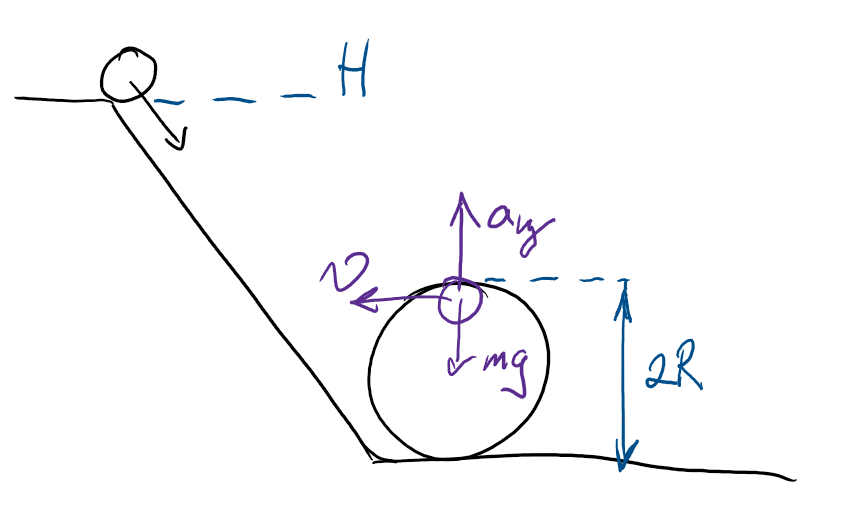
\includegraphics[height=5cm]{physics1/images/physics1_2024_10_21_1}
        \end{wrapfigure}
        
        Условие прохождения шара по мертвой петле: 
        
        $mg = a_{\text{ц}} = \frac{mv^2}{R} \quad \Longrightarrow \quad v = \sqrt{gR}$

        Кинетическая энергия в верхней точке петли: 
        
        $E_\text{к} = \frac{mv^2}{2} + \frac{I\omega^2}{2}$

        Шар катится без скольжения, значит имеет место быть вращательное движение, момент инерции для полнотелого шара $I = \frac{2}{3}mr^2$

        Получаем $mgH = 2mgR + \frac{mv^2}{2} + \frac{I\omega^2}{2} = 2mgR + \frac{mv^2}{2} + \frac{1}{3}mr^2 \cdot \frac{v^2}{r^2} = 
        2mgR + \frac{5}{6}mv^2$

        $h = 2R + \frac{5v^2}{6g} = 2R + \frac{5}{6}R = \frac{17}{6}R$
    \end{minipage}

\end{document}

